\centerline{\bf Комбинаторика 2}
\begin{enumerate}
\item Сколькими способами можно выбрать 3 ингридиента из 8 имеющихся, чтобы, возможно, получить филосовский
камень? Неважно, в каком порядке добавлять ингридиенты.
\item Сколькими способами можно выбрать $k$-элементное подмножество из \\ $n$-элементного множества, если порядок
выбираемых элементов не важен? (Не важно, какой элемент выбрали первым, а какой вторым). {\small Выведите
общую формулу, а затем формулу, записанную без многоточий. (если в вашей формуле есть многоточия)}

\definement{} Количество способов выбрать $k$ элементов из $n$ (то, что было посчитано в предыдущей
задаче) – $C_n^k$ (читается как Цэ из эн по ка). \\Иногда это называют числами сочетаний. Альтернативное обозначение $\vii{n}{k}$.

В следующих 3 задачах рекомендуется пользоваться смыслом $C_n^k$, описанным в определении (а не
формулой)

\item $ C_5^3 = \;?; \quad C_4^2 = \;?; \quad C_n^0 = \;?; \quad C_n^1 = \;?; \quad C_n^k - C_n^{n - k}
= \;?$

\item Чему равно значение суммы: $\sum_{k=0}^{n} C_n^k$?

\item Чему равно $C_n^k - C_{n - 1}^{k - 1}$?

\item Чему равен коэффициент при $a^k$ в выражении $(1 + a)^n$? Полученный результат увидел Ньютон, а
это выражение называется биномом Ньютона.

\item Чему равно значение суммы: $\sum_{k=0}^{\lfloor \frac{n}{2}\rfloor} C_n^{2k}$?

\begin{minipage}{0.6\textwidth}
\item Лягушка хочет добраться из верхнего ряда в нижний. При этом она может перемещаться либо вниз,
либо влево-вниз. Сколькими способами она может это сделать? (на картинке изображён один из способов,
а верхний и нижний ряды отмечены серым).
\end{minipage}
\begin{minipage}{0.3\textwidth}
\rightline{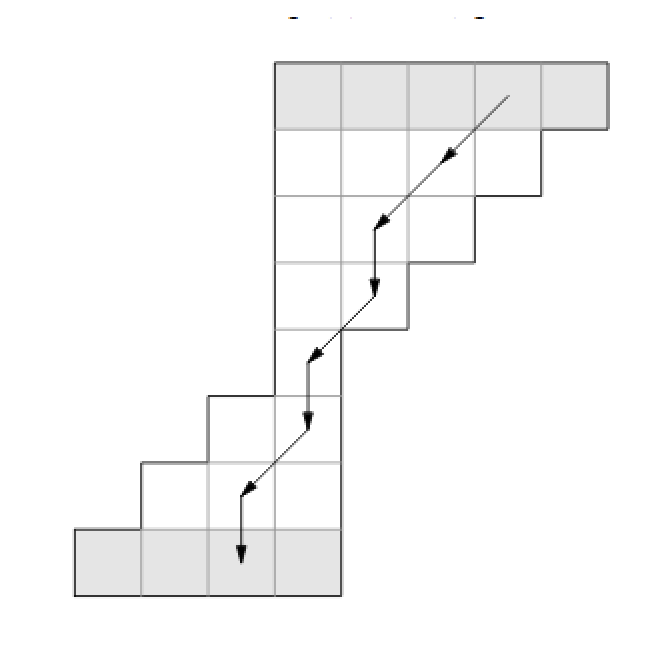
\includegraphics[width=1\linewidth]{K2-8.eps}}
\end{minipage}
\end{enumerate}
